\documentclass[a4paper,titlepage]{article}

\makeatletter
\def\input@path{{../../../template/}{./img}}
\makeatother

\usepackage{Comandi}
\usepackage{Riferimenti}
\usepackage{Stile}

\usepackage{comment}

% mi serve nella sezione Pianificazione. Mette "Attività" centrato sotto al processo
\newcommand{\att}{
	\begin{center}
	\textbf{Attività}
	\end{center}
	}

% mi serve nella sezione preventivo per mettere i grafici a torta. #1=path immagine, #2=caption
\newcommand{\torta}[2]{
	\begin{figure}[h]
		\centering
		\includegraphics[height=8cm, width=14cm]{#1} 
		\caption{#2}
	\end{figure}		
}




\def\NOME{Piano di Progetto}
\def\VERSIONE{0.1}
\def\DATA{\today}
\def\REDATTORE{Viviana Alessio}
\def\VERIFICATORE{Andrea Grendene}
\def\RESPONSABILE{Viviana Alessio}
\def\USO{Esterno}
\def\DESTINATARI{\COMMITTENTE \\ & \CARDIN \\ & \PROPONENTE}
\def\SOMMARIO{Piano per la per la gestione dei rischi, dei costi e dei tempi nella realizzazione del progetto del gruppo Beacon Strips.}


\begin{document}

\maketitle

\begin{diario}
	\modifica{Viviana Alessio}{\RES}{Sezione Pianificazione: Stesura fasi da PA a V}{2016-03-26}{0.3.3}
	\modifica{Viviana Alessio}{\RES}{Sezione Pianificazione: miglioramento organizzazione, Stesura fase AD}{2016-03-25}{0.3.2}
	\modifica{Viviana Alessio}{\RES}{Stesura Pianificazione: introduzione, fase A}{2016-03-23}{0.3.1}
	\modifica{Viviana Alessio}{\RES}{Stesura Analisi dei rischi: livello personale e organizzativo}{2016-03-23}{0.3.0}
	\modifica{Viviana Alessio}{\RES}{Stesura Analisi dei rischi: livello tecnologico}{2016-03-22}{0.2.1}
	\modifica{Viviana Alessio}{\RES}{Stesura Introduzione}{2016-03-16}{0.2.0}
	\modifica{Viviana Alessio}{\RES}{Stesura intestazione e indice documento}{2016-03-16}{0.1.0}
\end{diario}

\newpage
\tableofcontents
\newpage
\listoftables

\newpage

\section{Introduzione}
	\subsection{Scopo del documento} 
	Questo documento ha lo scopo di spiegare dettagliatamente le strategie secondo cui il gruppo \AUTORE{} intende condurre il \gl{progetto} didattico. 
	\subsection{Scopo del \gl{prodotto}}
	\SCOPO
	\subsection{Glossario}
	\GLOSSARIO
	\subsection{Riferimenti}
		\subsubsection{Normativi}
			\begin{itemize}
				\item \textbf{Capitolato d'appalto C2 - CLIPS:} Communication \& Localisation with Indoor Positioning Systems. \\
				\url{http://www.math.unipd.it/~tullio/IS-1/2015/Progetto/C2.pdf}
				\item \textbf{Vincoli e dettagli tecnico-economici} \\
				\url{http://www.math.unipd.it/~tullio/IS-1/2015/Dispense/PD01.pdf}
				\item \textbf{Norme di Progetto} \\ \NPdoc
				\item \textbf{Regolamento di Progetto} \\
				\url{http://www.math.unipd.it/~tullio/IS-1/2015/Progetto/}
				\item \textbf{Regolamento organigramma} \\
				\url{http://www.math.unipd.it/~tullio/IS-1/2015/Progetto/PD01b.html}
			\end{itemize}	
			
		\subsubsection{Informativi}
			\begin{itemize}
				\item \textbf{Software Engineering (10th edition}) \\
				Ian Sommerville \\
				Pearson Education | Addison-Wesley
				\item \textbf{Guide to the Software Engineering Body of Knowledge}
				IEEE Computer Society. Software Engineering Coordinating Committee
				\item \textbf{Slides del \COMMITTENTE} \\ riguardo i  \href{http://www.math.unipd.it/~tullio/IS-1/2015/Dispense/L02.pdf}{processi \gl{software}}, il \href{http://www.math.unipd.it/~tullio/IS-1/2015/Dispense/L03.pdf}{ciclo di vita del \gl{software}} e \href{http://www.math.unipd.it/~tullio/IS-1/2015/Dispense/L04.pdf}{la gestione di \gl{progetto}}	
			\end{itemize}
	\subsection{Modello di ciclo di vita scelto}
	È stato scelto come ciclo di vita il modello \gl{incrementale}. Le motivazioni che ci hanno spinto verso questa direzione sono il modo in cui è strutturato il \gl{progetto} didattico e la quasi totale inesperienza dei componenti del gruppo nello sviluppare progetti \gl{software} di grandi dimensioni. Di seguito una lista di caratteristiche del metodo \gl{incrementale}:
	\begin{itemize}
		\item si può produrre valore ad ogni incremento;
		\item ogni incremento riduce il rischio di fallimento;
		\item prevede rilasci multipli;
		\item i requisiti utente sono classificati e trattati in base alla loro importanza strategica. I requisiti più importanti sono già stabili all'inizio dello sviluppo del \gl{progetto};
		\item l'analisi dei requisiti e la progettazione architetturale non vengono ripetute;
		\item prima si pensa allo sviluppo dei requisiti essenziali, poi a quelli desiderabili;
		\item Sono presenti delle iterazioni del tipo Prototipo $\rightarrow$ Validazione $\rightarrow$ Prototipo $\rightarrow$ Validazione $\rightarrow$ ecc..
	\end{itemize}
	\subsection{Scadenze}
	Il gruppo Beacon Strips ha deciso di rispettare le seguenti scadenze:
	\begin{itemize} 
		\item \textbf{Revisione dei Requisiti}: 2016-04-18
		\item \textbf{Revisione di Progettazione}: 2016-06-17
		\item \textbf{Revisione di Qualifica}: 2016-08-24
		\item \textbf{Revisione di Accettazione}: 2016-09-12
	\end{itemize}
	In base a queste scadenze e a fronte dell'analisi dei rischi verranno decise le fasi in cui suddividere il lavoro di sviluppo del \gl{progetto}.
	\subsubsection{Scelta Revisione di Progettazione}
	Si è deciso di affrontare la RP$_{\mbox{\textit{min}}}$. Il gruppo si impegna quindi per il 2016-06-17 di presentare nel documento ``Specifica Tecnica'' la progettazione ad alto livello del \gl{prodotto}.
	

\section{Analisi dei rischi}
\label{analisiRischi}
	È stata attuata una profonda analisi dei rischi. In questo modo saremo pronti ad affrontarli in caso si presentassero.
	Ogni rischio è stato analizzato seguendo questa scaletta:
	\begin{enumerate}
		\item \textbf{Identificazione}: individuazione dei possibili rischi che si potranno riscontrare durante lo sviluppo del \gl{progetto}.
		\item \textbf{Analisi}: verrà analizzata la probabilità che i rischi si verifichino e come questi potrebbero influire sul lavoro;
		\item \textbf{Pianificazione di controllo}: verranno delineati i metodi grazie ai quali si cercherà di evitare che il rischio si verifichi;
		\item \textbf{Tecniche di mitigazione}: verranno delineati i metodi grazie ai quali verranno mitigati i rischi, nel caso si presentassero.
	\end{enumerate}
	Per ogni rischio verranno riportate le seguenti informazioni:
	\begin{itemize}
		\item \textbf{descrizione};
		\item \textbf{metodi di identificazione};
		\item \textbf{possibilità che si verifichi};
		\item \textbf{pericolosità};
		\item \textbf{conseguenze};
		\item \textbf{contromisure};
		\item \textbf{riscontro effettivo}.
	\end{itemize}

	\subsection{Livello tecnologico}
		\subsubsection{Uso di tecnologie e strumenti}
			\begin{itemize}
				\item \textbf{Descrizione}: alcune tecnologie e alcuni strumenti che verranno utilizzati sono sconosciuti ad alcuni membri del gruppo, altri sono sconosciuti a tutti i membri del gruppo;
				\item \textbf{Metodi di identificazione}: ogni componente del gruppo sarà consapevole delle proprie conoscenze e dei propri limiti in fase di apprendimento;
				\item \textbf{Possibilità che si verifichi}: alta;
				\item \textbf{Pericolosità}: alta;
				\item \textbf{Conseguenze}: rallentamento generale nell'avanzamento del \gl{progetto};
				\item \textbf{Contromisure}:  per evitare che il rischio si presenti ognuno si occuperà di studiare la tecnologia o lo strumento che ha intenzione di usare. Qualora un membro riscontrasse difficoltà con una tecnologia o uno strumento dovrà chiedere aiuto al \RES{} o ad uno degli Amministratori i quali gli forniranno quanto richiesto in forma scritta o verbale;
				\item \textbf{Riscontro effettivo}:
				\begin{itemize}
					\item \textbf{Periodo di Analisi e Management:} i membri del team hanno studiato e testato gli strumenti da utilizzare e non si è riscontrato alcun rallentamento significativo alla progettazione;
					\item \textbf{Periodo di Analisi di Dettaglio:} i membri del team hanno studiato e testato gli strumenti da utilizzare e non si è riscontrato alcun rallentamento significativo alla progettazione;
					\item \textbf{Periodo di Progettazione Architetturale:} i membri del team hanno studiato e testato gli strumenti da utilizzare e non si è riscontrato alcun rallentamento significativo alla progettazione;
               \item \textbf{Periodo di Progettazione di Dettaglio e Codifica:} ci sono state alcune lievi difficoltà legate agli strumenti da usare in fase di codifica (in particolare nell'acquisire sufficiente dimestichezza con l'editor \gl{Android Studio}) ma sono state superate in tempi brevi dall'intero gruppo.
				\end{itemize}
			\end{itemize}

		\subsubsection{Danneggiamento strumentazione \gl{hardware}}
			\begin{itemize}
				\item \textbf{Descrizione}: è possibile che i personal computer o altri strumenti in uso dal team subiscano danneggiamenti accidentali.
				\item \textbf{Metodi di identificazione}: ogni membro del gruppo dovrà essere consapevole del funzionamento o meno della strumentazione che possiede e$/$o che ha in uso;
				\item \textbf{Possibilità che si verifichi}: bassa;
				\item \textbf{Pericolosità}: alta;
				\item \textbf{Conseguenze}: rallentamento del lavoro che il proprietario$/$fruitore dello strumento danneggiato dovrebbe svolgere;
				\item \textbf{Contromisure}: non è possibile prevedere danneggiamenti \gl{hardware}, ma per evitare perdite di lavoro ogni componente del gruppo al termine di una sessione di lavoro si occuperà di fare una \gl{commit} sulla \gl{repository}. Nel caso si verifichino danni \gl{hardware} il proprietario$/$fruitore dovrà, se possibile, preoccuparsi di aggiustare lo strumento danneggiato o di procurarne uno sostitutivo. Se lo considererà necessario potrà chiedere aiuto ad uno degli Amministratori;
				\item \textbf{Riscontro effettivo}:
				\begin{itemize}
					\item \textbf{Periodo di Analisi e Management:} non c'è stato alcun guasto di strumentazione hardware all'interno del team;
					\item \textbf{Periodo di Analisi di Dettaglio:} non c'è stato alcun guasto di strumentazione hardware all'interno del team;
					\item \textbf{Periodo di Progettazione Architetturale:} non c'è stato alcun guasto di strumentazione hardware all'interno del team;
               \item \textbf{Periodo di Progettazione di Dettaglio e Codifica:} sì è verificato un guasto grave al PC di un componente del gruppo che è diventato quindi inutilizzabile. Fortunatamente il proprietario ha trovato in tempi brevi (3 giorni) un computer sostituto e il sistema di sviluppo basato su repository remota ha consentito di non perdere pressoché alcun dato legato al progetto.
               Il rallentamento a ciò dovuto è stato assorbito dal componente, nei giorni seguenti, senza impattare le scadenze complessive del team.
				\end{itemize}
			\end{itemize}

		\subsubsection{Problemi \gl{software} strumenti utilizzati}
		\begin{itemize}
			\item \textbf{Descrizione}: è possibile che gli strumenti scelti per agevolare i processi abbiano problemi di varia natura;
			\item \textbf{Metodi di identificazione}: chi utilizza uno strumento che sembra causare problemi lo farà presente ad un \AM{} che si occuperà di verificare la reale esistenza del problema;
			\item \textbf{Possibilità che si verifichi}: media;
			\item \textbf{Pericolosità}: alta;
			\item \textbf{Conseguenze}: forte rallentamento del lavoro;
			\item \textbf{Contromisure}: non è possibile evitare a priori che si verifichino problemi con il SW. Nel caso questi problemi si presentassero gli Amministratori dovranno estinguere il problema se il SW che causa problemi è stato creato dal team, altrimenti provvederà a trovare uno strumento alternativo che faccia un lavoro migliore di quello che causa problemi;
			\item \textbf{Riscontro effettivo}:
			\begin{itemize}
				\item \textbf{Periodo di Analisi e Managment:} si sono riscontrate difficoltà nell'installazione del software Trender all'interno del server dato in dotazione da \PROPONENTE, le quali sono state successivamente risolte contattando il produttore e intervenendo sul codice sorgente. Non si sono riscontrati ritardi significativi nell'avanzamento della progettazione;
				\item \textbf{Periodo di Analisi di Dettaglio:} non si sono riscontrati problemi di questo tipo;
				\item \textbf{Periodo di Progettazione Architetturale:} non si sono riscontrati problemi di questo tipo;
            \item \textbf{Periodo di Progettazione di Dettaglio e Codifica:} non si sono riscontrati problemi di questo tipo.
			\end{itemize}
		\end{itemize}


	\subsection{Livello personale}
	\label{sez2.2}
		\subsubsection{Problemi personali dei componenti}
		\begin{itemize}
			\item \textbf{Descrizione}: ogni membro del gruppo ha impegni relativi alla propria vita privata che potrebbero incidere sulla pianificazione delle attività;
			\item \textbf{Metodi di identificazione}: il \RES{} verrà informato tempestivamente se si presenteranno impegni personali non precedentemente comunicati;
			\item \textbf{Possibilità che si verifichi}: media;
			\item \textbf{Pericolosità}: media;
			\item \textbf{Conseguenze}: rallentamento del lavoro individuale o, in casi più gravi, rallentamento del lavoro dell'intero gruppo;
			\item \textbf{Contromisure}: ogni membro del gruppo dichiarerà all'inizio del \gl{progetto} i propri impegni personali al \RES{} tenendo conto anche dei possibili impegni extra che riesce a prevedere. Nel caso in cui un impegno personale rallenti un membro del gruppo per molto tempo il \RES{} sposterà in avanti le scadenze prefissate, se questo sarà possibile. In alternativa il \RES{} si occuperà di incaricare un altro membro del gruppo a svolgere il lavoro di chi non può farlo;
			\item \textbf{Riscontro effettivo}:
			\begin{itemize}
				\item \textbf{Periodo di Analisi e Management:} non si sono riscontrati problemi di questo tipo;
				\item \textbf{Periodo di Analisi di Dettaglio:} Tommaso è stato impegnato in un lavoro extra-curricolare che lo ha sottratto a qualche ora di attività di \AN; grazie alla sua segnalazione si è deciso di assegnare le ore mancanti ad altri componenti del team provvedendo a farle recuperare a Tommaso nei periodi successivi.
				\item \textbf{Periodo di Progettazione Architetturale:} l'impegno lavorativo extra-curricolare di Tommaso è proseguito anche in questa fase. Data la minore disponibilità di Tommaso si è deciso di:
					\begin{itemize}
						\item cambiare il ruolo di \RES {} da Tommaso a Matteo; Tommaso sarà quindi responsabile nella prossima fase, in quanto l'impegno lavorativo aggiuntivo non sarà più presente;
						\item cambiare il ruolo di quarto \PRJ {} da Tommaso a Viviana;
						\item assegnare a Tommaso i ruoli di \VER{} e \AN.
					\end{itemize}
            \item \textbf{Periodo di Progettazione di Dettaglio e Codifica:} alcuni membri hanno trascorso qualche giorno di ferie: in complesso ci sono stati 8 giorni di inattività (tra vari componenti) nei mesi di luglio e agosto che sono stati in seguito recuperati con un maggior impegno al rientro.
			\end{itemize}
		\end{itemize}


		\subsubsection{Problemi tra i componenti}
		\begin{itemize}
			\item \textbf{Descrizione}: il gruppo è formato da sei persone ed è possibile che in certi momenti del \gl{progetto} sorgano disaccordi e discussioni;
			\item \textbf{Metodi di identificazione}: chi ha problemi con uno o più membri del gruppo deve comunicarlo tempestivamente al \RES{};
			\item \textbf{Possibilità che si verifichi}: bassa;
			\item \textbf{Pericolosità}: media;
			\item \textbf{Conseguenze}: svogliatezza nello svolgere i compiti assegnati, ritardo nel portare a termine tali compiti;
			\item \textbf{Contromisure}: ogni membro del gruppo si impegnerà ad essere disponibile a discussioni costruttive e cercherà di non generare litigi insensati. Qualora questi ultimi sorgessero il \RES{} si occuperà di placare gli animi.
			\item \textbf{Riscontro effettivo}:
			\begin{itemize}
				\item \textbf{Periodo di Analisi e Management:} non si sono riscontrati problemi di questo tipo;
				\item \textbf{Periodo di Analisi di Dettaglio:} non si sono riscontrati problemi di questo tipo;
				\item \textbf{Periodo di Progettazione Architetturale:} non si sono riscontrati problemi di questo tipo;
            \item \textbf{Periodo di Progettazione di Dettaglio e Codifica:} non si sono riscontrati problemi di questo tipo.
			\end{itemize}
		\end{itemize}

	\subsection{Livello organizzativo}
		\subsubsection{Errori nella valutazione dei tempi e dei costi}
		\begin{itemize}
			\item \textbf{Descrizione}: è possibile che durante la stesura della pianificazione venga commesso qualche errore riguardo i tempi e i costi dovuto all'inesperienza;
			\item \textbf{Metodi di identificazione}: qualora qualcuno si accorgesse di discrepanze rispetto alla pianificazione deve prontamente notificarlo al \RES{}. Quest'ultimo dovrà assicurarsi, in ogni caso, che lo svolgimento delle attività prosegua secondo i piani;
			\item \textbf{Possibilità che si verifichi}: alta;
			\item \textbf{Pericolosità}: alta;
			\item \textbf{Conseguenze}: rallentamento nell'ultimazione delle attività pianificate;
			\item \textbf{Contromisure}: ogni membro del gruppo si impegnerà per rispettare le consegne assegnategli. Colui che assegna i \gl{tasks} ai membri del gruppo dovrà tenere conto di possibili ritardi e calcolare che questi non compromettano il lavoro del resto del gruppo;
			\item \textbf{Riscontro effettivo}:
			\begin{itemize}
				 \item \textbf{Periodo di Analisi e Managment} il team non era a conoscenza che la consegna dell'offerta tecnico-economica fosse anticipata (1 Aprile), rispetto alla data di consegna della documentazione per la RP (11 Aprile). Insieme ai team che si trovavano nella nostra stessa condizione si è deciso di segnalare, tramite una mail comune, il problema al Committente, il quale ha posticipato la data (7 Aprile); questo evento ha prodotto un'accelerazione nell'ultimazione dei documenti, non creando però gravi conseguenze;
				 \item \textbf{Periodo di Analisi di Dettaglio}: sono stati necessari più giorni di quelli inizialmente pianificati per sistemare soddisfacentemente il lavoro di analisi dei requisiti. Conseguentemente si è dovuto accorciare il periodo di Progettazione Architetturale;
				 \item \textbf{Periodo di Progettazione Architetturale:} nonostante questo periodo sia stato leggermente ridotto il team è riuscito a rispettare le ore preventivate;
             \item \textbf{Periodo di Progettazione di Dettaglio e Codifica:} il team è riuscito a rispettare le ore preventivate.
			\end{itemize}
		\end{itemize}


		\subsubsection{Problemi di comprensione dei requisiti}
		\begin{itemize}
			\item \textbf{Descrizione}: è possibile che durante l'analisi dei requisiti alcuni aspetti vengano compresi in modo incompleto o, addirittura, errato. Questo sempre a causa dell'inesperienza del gruppo;
			\item \textbf{Metodi di identificazione}: se sorgeranno dubbi riguardo i requisiti ci si accorderà con il Proponente sulla strada giusta da seguire;
			\item \textbf{Possibilità che si verifichi}: media;
			\item \textbf{Pericolosità}: bassa;
			\item \textbf{Conseguenze}: rallentamento del lavoro, possibilità di mancanza di requisiti fondamentali.
			\item \textbf{Contromisure}: non sono state identificate contromisure efficaci se non il prestare particolare attenzione a quanto detto dal Proponente durante le riunioni sostenute;
			\item \textbf{Riscontro effettivo}:
			\begin{itemize}
				\item \textbf{Periodo di Analisi e Managment}: si è discusso di alcuni dubbi sui requisiti del progetto con il Proponente durante gli incontri effettuati facilitando la parte iniziale dell'analisi dei requisiti;
				\item \textbf{Periodo di Analisi di Dettaglio:} non si sono verificati ulteriori problemi di questo tipo;
				\item \textbf{Periodo di Progettazione Architetturale:} non si sono verificati ulteriori problemi di questo tipo;
            \item \textbf{Periodo di Progettazione di Dettaglio e Codifica:} non si sono verificati problemi di questo tipo.
			\end{itemize}
		\end{itemize}

      \subsubsection{Problemi di reperimento di un luogo dove trovarsi}
		\begin{itemize}
			\item \textbf{Descrizione}: è possibile che il gruppo abbia necessita di trovarsi di persona e che i luoghi comunemente adibiti, come le aule fuori dagli orari di lezione oppure le aule studio, non siano disponibili;
			\item \textbf{Metodi di identificazione}: qualora il gruppo avesse la necessità di trovarsi di persona ma non si riuscisse a trovare un luogo.
			\item \textbf{Possibilità che si verifichi}: perlopiù bassa, alta in luglio$/$agosto;
			\item \textbf{Pericolosità}: bassa;
			\item \textbf{Conseguenze}: rallentamento del lavoro, difficoltà nel chiarire incomprensione, possibilità di fraintendimenti;
			\item \textbf{Contromisure}: intensificare la comunicazione attraverso Slack, sopperire all'incontro di persona con delle video-conferenze con \gl{Hangout}, eventualmente trovare qualche altro luogo dove riunirsi;
			\item \textbf{Riscontro effettivo}:
			\begin{itemize}
				\item \textbf{Periodo di Analisi e Managment}: non si sono verificati problemi di questo tipo;
				\item \textbf{Periodo di Analisi di Dettaglio:} non si sono verificati problemi di questo tipo;
				\item \textbf{Periodo di Progettazione Architetturale:} non si sono verificati problemi di questo tipo;
            \item \textbf{Periodo di Progettazione di Dettaglio e Codifica:} il problmea si è verificato con il periodo di chiusura estivo delle aule (mediamente dal 23 luglio al 21 agosto), ma il team ha sopperito efficaciemente al problema con diverse chiamate di gruppo su \gl{Google Hangout}.
			\end{itemize}
		\end{itemize}


\section{Pianificazione} 
\label{pianificazione}
	\subsection{Introduzione}
	A fronte dell'analisi dei rischi e della scadenza delle revisioni di avanzamento vi saranno tre periodi durante lo svolgimento del \gl{progetto}: uno di \textbf{analisi}, uno di \textbf{progettazione e codifica} ed uno di \textbf{incremento e validazione}.
	Per rendere più controllabile lo sviluppo del \gl{progetto} si è deciso di dividere il lavoro in sei periodi specifici, i quali vengono riportati nella seguente tabella con le relative date di inizio e di fine.
		
		\begin{tabella}{!{\VRule}c!{\VRule}c!{\VRule}c!{\VRule}c!{\VRule}} %date non standard \gl{ISO}
				
			\intestazionethreecol{Periodo}{Data di inizio}{Data di fine}
			
			Periodo di Analisi e Management & 2016-03-01 & 2016-04-18  \\
			Periodo di Analisi di Dettaglio & 2016-04-19 & 2016-05-06  \\
			Periodo di Progettazione Architetturale & 2016-05-07 & 2016-06-17 \\
			Periodo di Progettazione di Dettaglio e Codifica & 2016-06-18 & 2016-08-24 \\
			Periodo di Codifica dei Requisiti Desiderabili e Opzionali & 2016-08-25 & 2016-08-30 \\
			Periodo di Validazione e Collaudo & 2016-08-31 & 2016-09-12 \\ 
			
			\hiderowcolors
			\caption{Periodi di sviluppo con relative abbreviazioni e date di inizio e fine.}
			
		\end{tabella}
		
	Ogni periodo contiene diverse attività che verranno riportate e descritte in un elenco puntato. \\ Successivamente nei diagrammi di \gl{Gantt} si potrà notare come le attività siano state suddivise temporalmente. In questi saranno inoltre presenti delle \gl{milestones} che indicheranno i giorni in cui dovranno essere consegnati i documenti in entrata alle revisioni, quelli in cui si svolgeranno le revisioni di avanzamento ed, eventualmente, quelli in cui vi saranno incontri con il Proponente. 
	
	\subsection{Periodo di Analisi e Management (AM)}
	\begin{center}
		\textbf{Data di inizio}: 2016-03-01 \\
		\textbf{Data di fine}: 2016-04-18 \\
	\end{center}

	Questo periodo inizia con la formazione del gruppo e termina il giorno della Revisione dei Requisiti. \\
	I processi principali di questo periodo sono: 
	\begin{itemize}
		\item \textbf{Management}
			\att
			\begin{itemize} 
				\item \textbf{Individuazione strumenti da utilizzare}: il gruppo deve trovare degli strumenti che aiutino ad automatizzare e rendere più facile lo sviluppo del \gl{progetto}.
			\end{itemize}
		\item \textbf{Documentazione}: viene creata la documentazione da consegnare in ingresso alla RR.
		\att
		\begin{itemize}
			\item \textbf{Norme di Progetto}: viene steso il documento \NPdocRR{} in cui saranno elencate e descritte le norme da seguire durante tutto lo svolgimento del \gl{progetto} indipendentemente dal \gl{capitolato} scelto; 
			\item \textbf{Piano di Progetto}: viene steso il documento \PPdocRR{} per pianificare dettagliatamente i tempi e i costi del \gl{progetto};
			\item \textbf{Studio di Fattibilità}: viene steso il documento \SFdocRR{} che riporta l'analisi che ha portato il gruppo a scegliere il \gl{capitolato} C2;
			\item \textbf{Analisi dei Requisiti}: viene steso il documento \ARdocRR{} in cui viene svolta un'analisi molto più approfondita di quella svolta in \SFdocRR. Vengono elencati e descritti i casi d'uso e i requisiti del \gl{prodotto} che si andrà a sviluppare;
			\item \textbf{Piano di Qualifica}: viene steso il documento \PQdocRR{} che riporta quali obiettivi di qualità si è prefissato il gruppo;
			\item \textbf{Glossario}: viene steso il \GldocRR{} il quale riporta la descrizione dei termini presenti nei vari documenti che potrebbero causare ambiguità nel lettore.
		\end{itemize}
		\item \textbf{Sviluppo}
		\att
			\begin{itemize}
				\item \textbf{Analisi}: vengono identificati i requisiti ed i casi d'uso necessari per il successivo sviluppo dell'applicazione.
			\end{itemize}
		\item \textbf{Infrastruttura}
		\att 
		\begin{itemize}
			\item \textbf{Trender}: gli amministratori si occupano di configurare \gl{Trender} e renderlo funzionante.
		\end{itemize}
	\end{itemize}
	
		
		\subsubsection{Diagramma di \gl{Gantt} delle attività}
		% \gantt{img/gantt/A}{Diagramma di \gl{Gantt} delle attività - Periodo A}
		
		\begin{figure}[!h]
			\centering
			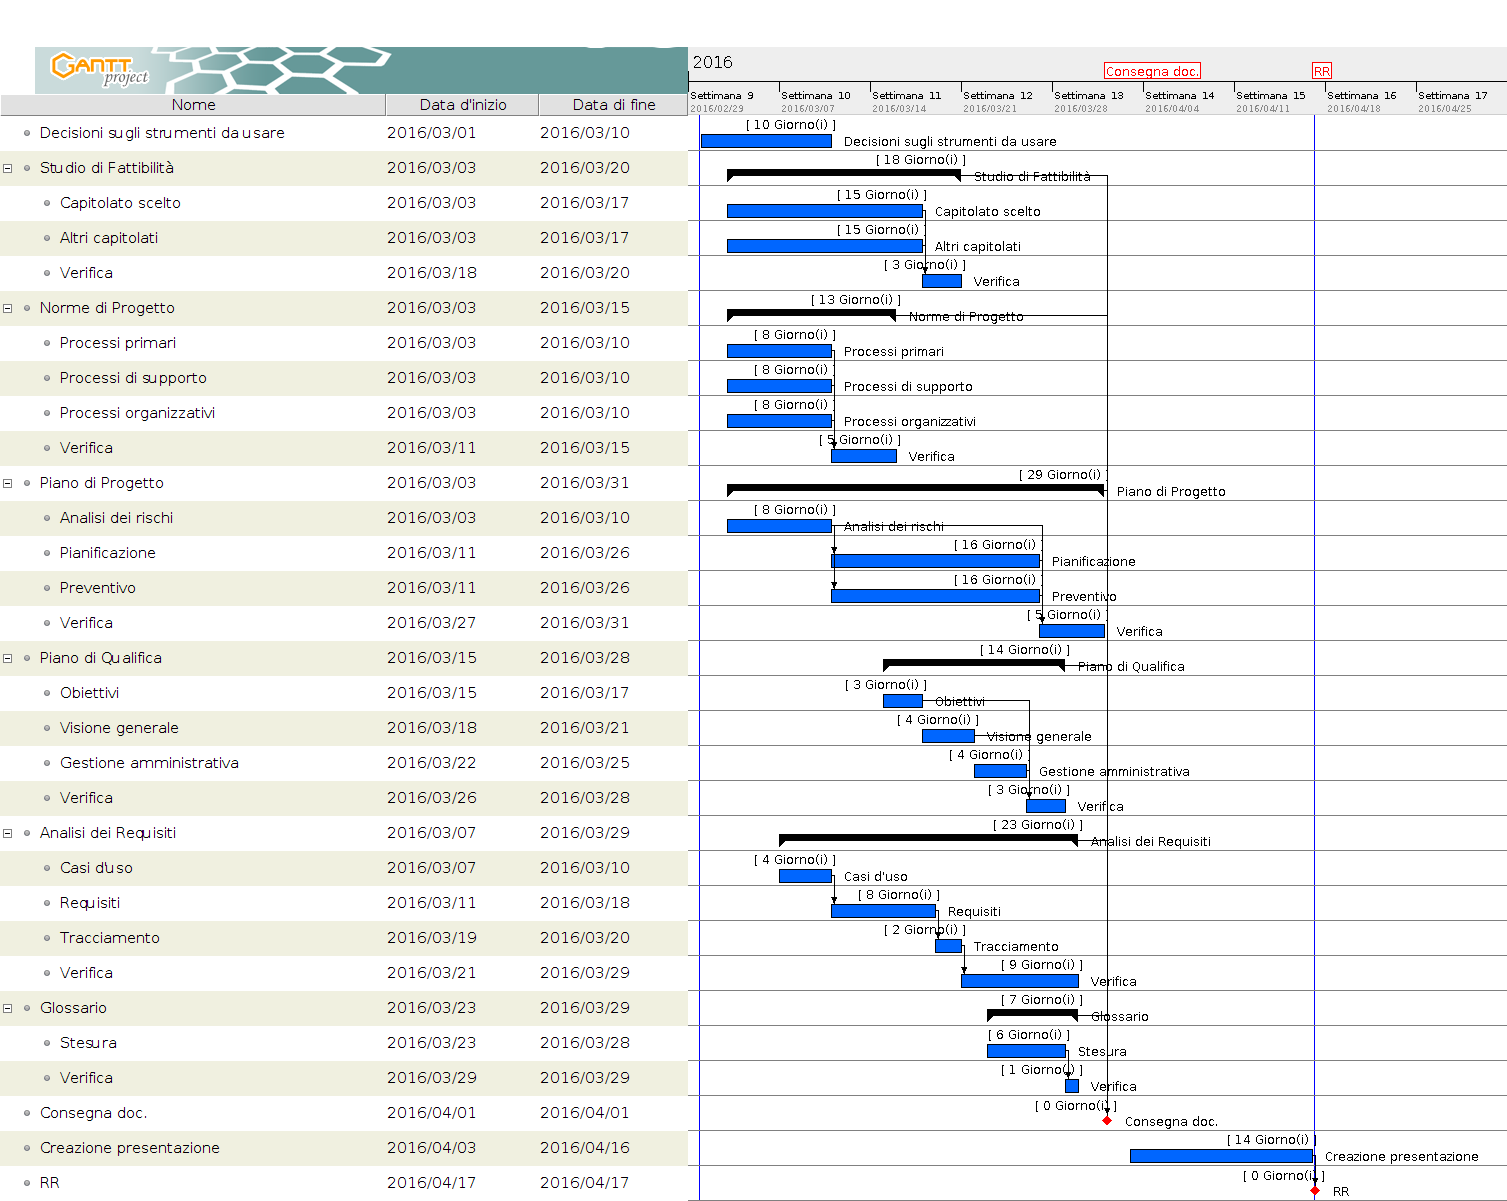
\includegraphics[height=12cm, width=15cm]{img/gantt/A} 
			\caption{Diagramma di \gl{Gantt} delle attività - Periodo di Analisi e Management}
		\end{figure}
		
	\subsection{Periodo di Analisi di Dettaglio (CR)}
	\begin{center}
		\textbf{Data di inizio}: 2016-04-19 \\
		\textbf{Data di fine}: 2016-05-06 \\
	\end{center}
	Questo periodo inizia al termine del periodo di Analisi e Management, ovvero dopo la Revisione dei Requisiti, e termina con un incontro con il \gl{proponente}. \\ 
	Il processo principale di questo periodo è:
	\begin{itemize}
		\item \textbf{Documentazione}
		\att
		\begin{itemize}
			\item \textbf{Miglioramento di tutti i documenti}: seguendo le indicazioni del Committente verranno attuate le modifiche necessarie a migliorare tutti i documenti stesi nel periodo di Analisi e Management;
			\item \textbf{Analisi dei Requisiti}: Questo documento oltre ad essere corretto verrà anche arricchito con nuovi requisiti.
		\end{itemize}
		\item \textbf{Sviluppo}
		\att
		\begin{itemize}
			\item \textbf{Analisi}: verranno corretti gli errori riguardo l'analisi effettuati nel periodo precedente. Successivamente, se necessario, ci si occuperà di proseguire con l'analisi aggiungendo nuovi requisiti e casi d'uso.
		\end{itemize}
	\end{itemize}
		
		
		\subsubsection{Diagramma di \gl{Gantt} delle attività}
		\gantt{img/gantt/AD}{Diagramma di \gl{Gantt} delle attività - Periodo di Analisi di Dettaglio}
		
	\subsection{Periodo di Progettazione Architetturale (PA)}
	\begin{center}
		\textbf{Data di inizio}: 2016-05-07 \\
		\textbf{Data di fine}: 2016-06-17 \\
	\end{center}
	Questo periodo inizia subito dopo il termine del periodo di Analisi di Dettaglio e termina con la data della Revisione di Progettazione. \\
	Il processo principale di questo periodo è:
		\begin{itemize}
			\item \textbf{Documentazione}
			\att
			\begin{itemize}
				\item \textbf{Specifica Tecnica}: viene creato il documento \STdocRP{} che conterrà le scelte progettuali decise dai progettisti; 
				\item \textbf{Norme di Progetto}: viene incrementato questo documento in modo da normare anche la stesura del documento \STdocRP;
				\item \textbf{Piano di Progetto}: viene aggiunto il consuntivo del periodo contenente i periodi di Analisi di Dettaglio e di Progettazione Architetturale ed il preventivo a finire. Vengono inoltre riportati i rischi che si sono verificati nei periodi precedenti;
				\item \textbf{Piano di Qualifica}: viene aggiunta la parte di pianificazione dei test;
				\item \textbf{Glossario}: viene incrementato con i nuovi termini presenti nella \STdocRP, nel \PQdocRP{} e nelle \NPdocRP.
			\end{itemize}
			\item \textbf{Sviluppo}
			\att
			\begin{itemize}
				\item \textbf{Progettazione}: verranno identificate ad alto livello le classi da utilizzare per la realizzazione dell'applicazione.
			\end{itemize}
			\item \textbf{\gl{Training}}
			\att
			\begin{itemize}
				\item \textbf{\gl{Android Studio}}: ogni componente del gruppo si occuperà di imparare ad utilizzare \gl{Android Studio}, in quanto questo strumento verrà utilizzato nella fase seguente per la codifica.
			\end{itemize}
		
		\end{itemize}
		\subsubsection{Diagramma di \gl{Gantt} delle attività}
		\gantt{img/gantt/PA}{Diagramma di \gl{Gantt} delle attività - Periodo di Progettazione Architetturale}
		
		
		
	\subsection{Periodo di Progettazione di Dettaglio e Codifica (PDC)}
	\begin{center}
		\textbf{Data di inizio}: 2016-06-18 \\
		\textbf{Data di fine}: 2016-08-24 \\
	\end{center}
	Questo periodo inizia subito dopo la fine del periodo di Progettazione Architetturale, ovvero dopo la Revisione di Progettazione, e termina con la data della Revisione di Qualifica. \\
	I processi principali di questo periodo sono: 
		\begin{itemize}
			\item \textbf{Documentazione} 
			\att
			\begin{itemize} 
				\item \textbf{Definizione di \gl{Prodotto}}: viene steso il documento \DPdocRQ{} il quale definisce la struttura e la relazione tra le componenti del \gl{prodotto}. È basato sul documento \STdocRQ;
				\item \textbf{Manuale utente}: viene redatta la versione preliminare del \MUdocRQ{} il quale fornirà agli utenti le indicazioni per l'utilizzo del \gl{prodotto};
				\item \textbf{Incremento altri documenti}: come nel periodo precedente anche in questa vi sarà il miglioramento dei documenti che necessitano tale trattamento.
			\end{itemize}
			\item \textbf{Sviluppo}
			\att
			\begin{itemize}
				\item \textbf{Codifica}: avviene la scrittura del codice dei requisiti obbligatori del \gl{prodotto};
				\item \textbf{Verifica}: per verificare l'efficacia del codice \gl{prodotto} nell'attività di codifica vengono eseguiti i test di unità e di integrazione e ne vengono osservati i risultati. 
			\end{itemize}
		\end{itemize}
		\subsubsection{Diagramma di \gl{Gantt} delle attività}
		% \gantt{img/gantt/PDC}{Diagramma di \gl{Gantt} delle attività - Periodo PDC}
		
		\begin{figure}[!h]
			\centering
			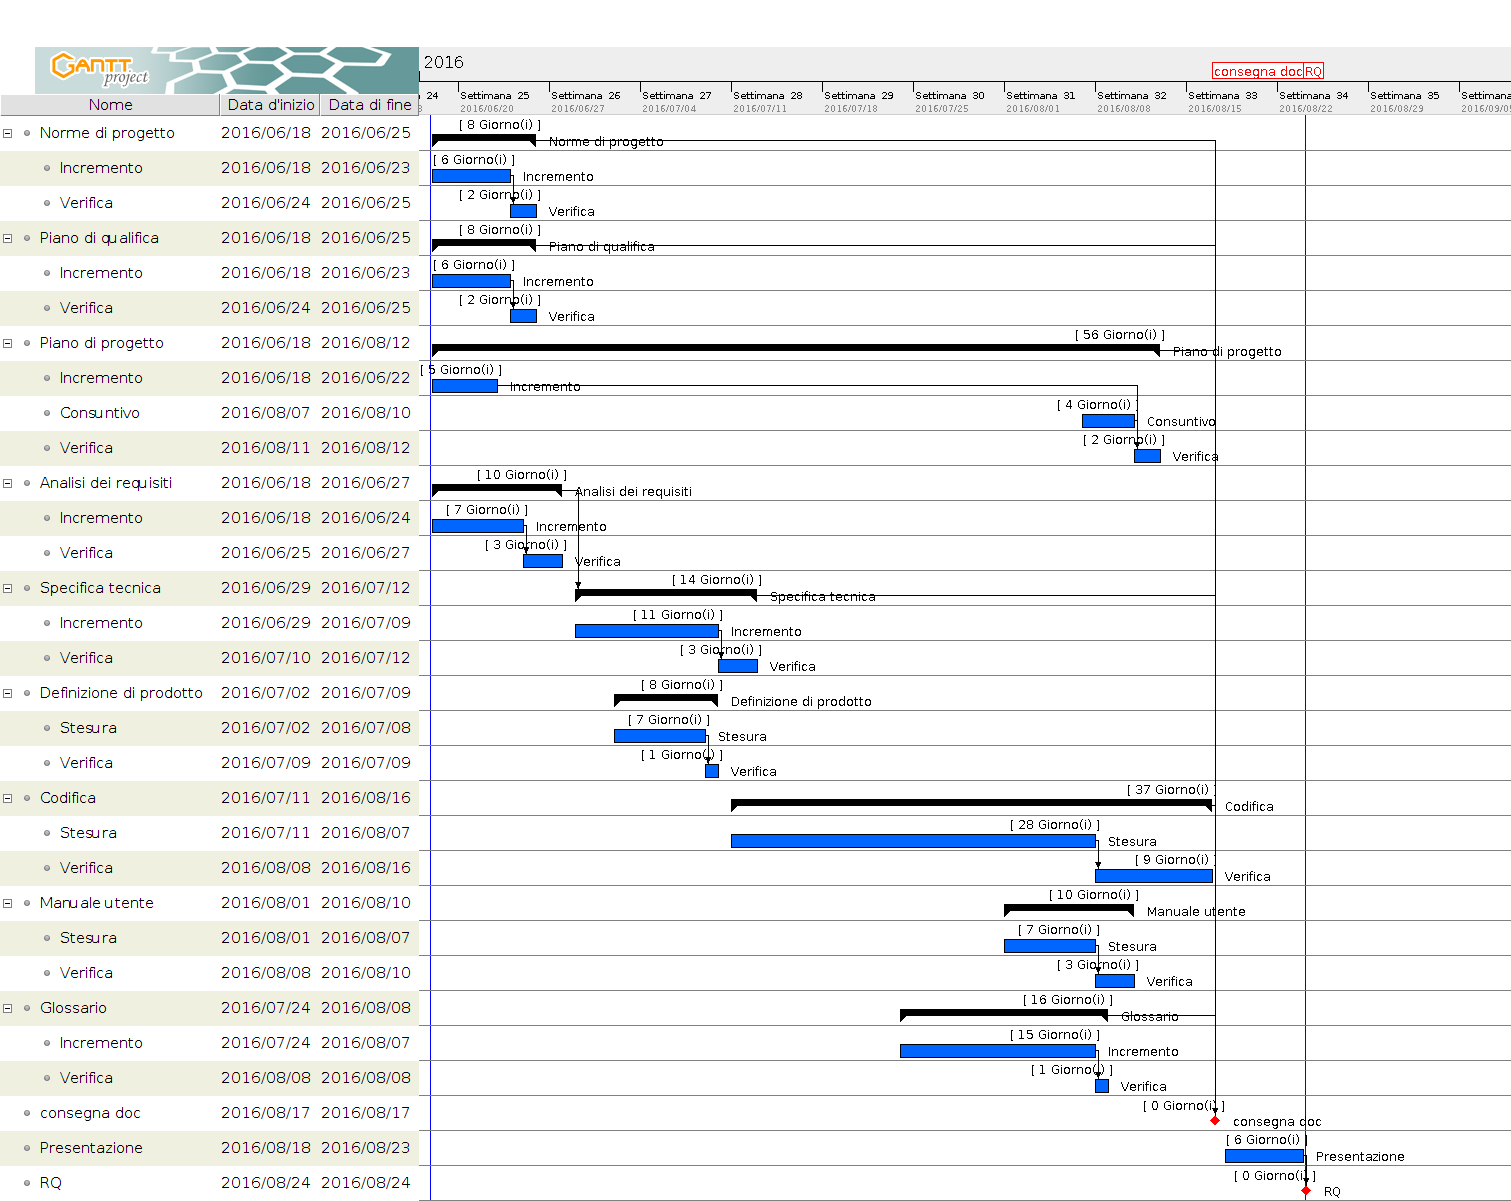
\includegraphics[height=12cm, width=15cm]{img/gantt/PDC} 
			\caption{Diagramma di \gl{Gantt} delle attività - Periodo di Progettazione di Dettaglio e Codifica}
		\end{figure}
		
	\subsection{Periodo di Codifica dei Requisiti Desiderabili e Opzionali (CDO)}
	\begin{center}
		\textbf{Data di inizio}: 2016-08-25 \\
		\textbf{Data di fine}: 2016-08-30 \\
	\end{center}
	Questo periodo inizia subito dopo la fine del periodo di Progettazione di Dettaglio e Codifica, ovvero dopo la Revisione di Qualifica, e termina sei giorni dopo. \\
	I processi principali di questo periodo sono: 
		\begin{itemize}
			\item \textbf{Documentazione}:
			\att
			\begin{itemize}
				\item \textbf{Correzioni e aggiornamenti}: Verranno corretti e aggiornati tutti i documenti che lo necessitano. 
			\end{itemize}
			\item \textbf{Sviluppo}:
			\att
			\begin{itemize}
				\item \textbf{Codifica}: avviene la scrittura del codice dei requisiti desiderabili e opzionali del \gl{prodotto};
				\item \textbf{Verifica}: per verificare l'efficacia del codice \gl{prodotto} nell'attività di codifica vengono eseguiti i test di unità e di integrazione e ne vengono osservati i risultati. 
			\end{itemize}
		\end{itemize}
		\subsubsection{Diagramma di \gl{Gantt} delle attività}
		% \gantt{img/gantt/RD}{Diagramma di \gl{Gantt} delle attività - Periodo RD}
		
		\begin{figure}[!h]
			\centering
			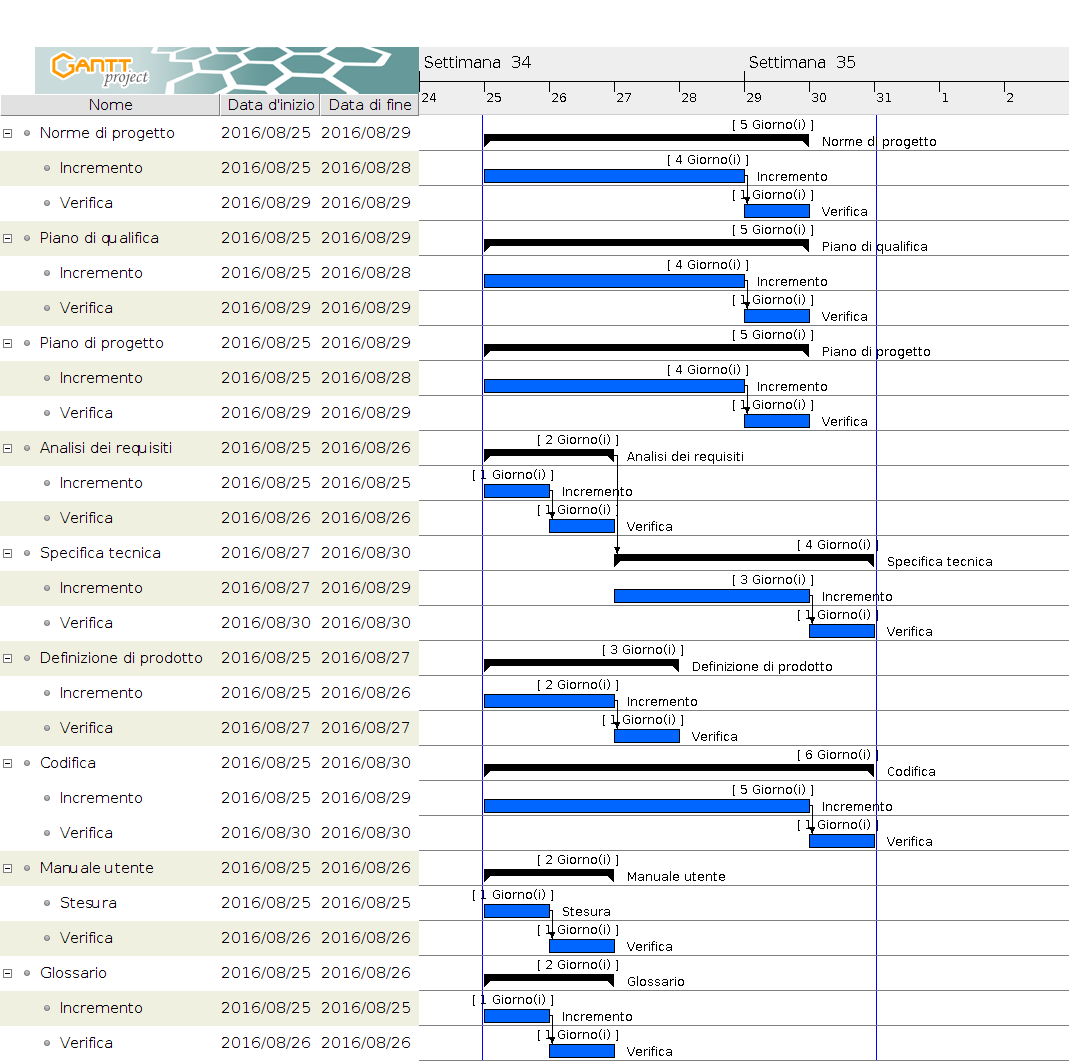
\includegraphics[height=12cm, width=15cm]{img/gantt/RD} 
			\caption{Diagramma di \gl{Gantt} delle attività - Periodo di Codifica dei Requisiti Desiderabili e Opzionali}
		\end{figure}
		
	\subsection{Periodo di Validazione e Collaudo (VC)}
	\begin{center}
		\textbf{Data di inizio}: 2016-08-31 \\
		\textbf{Data di fine}: 2016-09-12 \\
	\end{center}
	Questo periodo inizia subito dopo la fine del periodo di Codifica dei Requisiti Desiderabili e Opzionali e termina con la data della Revisione di Accettazione. \\
	I processi principali di questo periodo sono:
		\begin{itemize}
			\item \textbf{Documentazione}
			\att
			\begin{itemize}
				\item \textbf{Correzioni e aggiornamenti}: Verranno corretti e aggiornati tutti i documenti che lo necessitano. Si otterrà la versione finale della documentazione. 
			\end{itemize}
			\item \textbf{Sviluppo}
			\att
				\begin{itemize}
					\item \textbf{Test}: vengono eseguiti i test di sistema previsti e ne vengono osservati e monitorati i risultati. 
				\end{itemize}
			\item \textbf{Verifica e validazione}
			\att
			\begin{itemize}
				\item \textbf{Collaudo}: il \gl{prodotto} viene collaudato sulle funzionalità previste;
				\item \textbf{Verifica}: tramite tracciamento si verifica di aver soddisfatto i requisiti presenti nel documento \ARdocRA. Si verificheranno inoltre i canoni di qualità previsti nel \PQdocRA;
				\item \textbf{Validazione}: una volta svolte tutte le verifiche il \gl{prodotto} può considerarsi validato.
			\end{itemize}
		\end{itemize}
		\subsubsection{Diagramma di \gl{Gantt} delle attività}
		% \gantt{img/gantt/V}{Diagramma di \gl{Gantt} delle attività - Periodo V}
		
		\begin{figure}[!h]
			\centering
			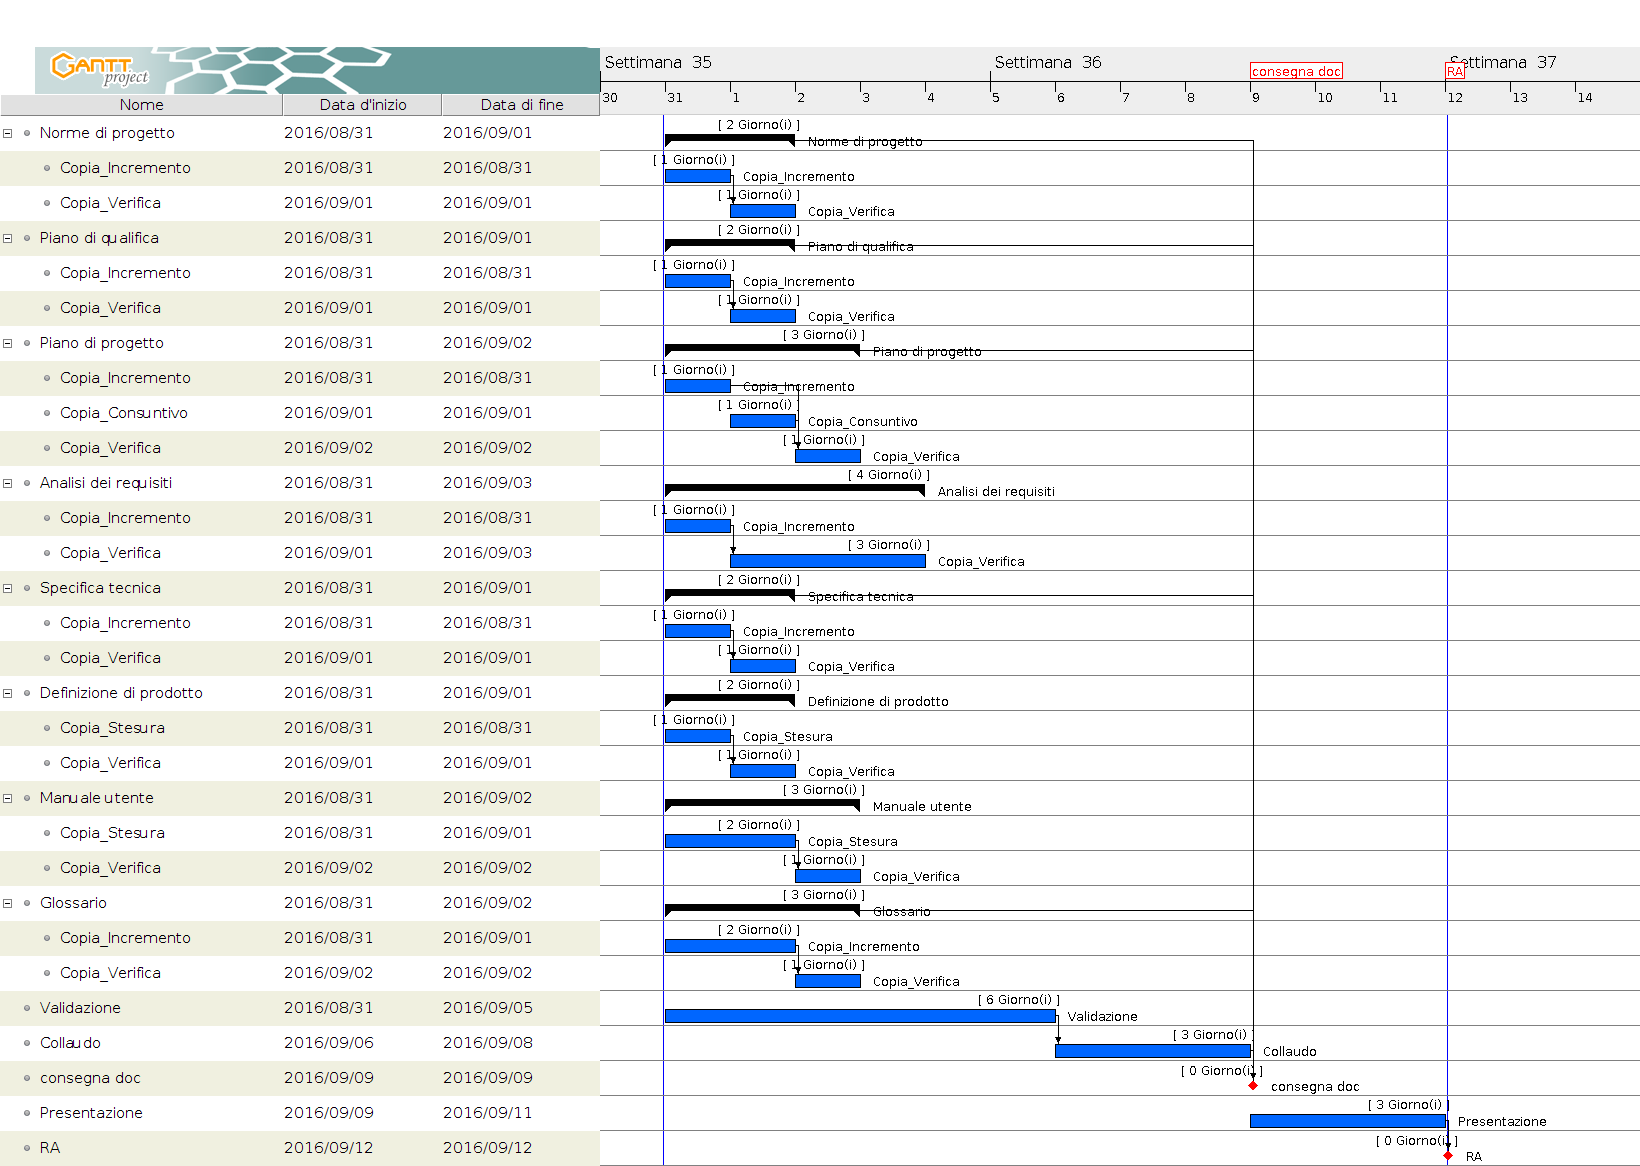
\includegraphics[height=11cm, width=15cm]{img/gantt/V} 
			\caption{Diagramma di \gl{Gantt} delle attività - Periodo di Validazione e Collaudo}
		\end{figure}


\section{Preventivo} 
	\subsection{Introduzione}
		A fronte della pianificazione sono stati decise per ogni fase quante ore ogni componente del gruppo dovrà svolgere per ruolo.
		Per favorire la rotazione dei ruoli sarà possibile che alcuni membri in una singola fase svolgano diversi ruoli. \\
		Nelle tabelle e in alcuni grafici si farà uso delle abbreviazioni seguenti per indicare i ruoli:
		\begin{itemize}
			\item RE: Responsabile;
			\item AM: Amministratore;
			\item AN: Analista;
			\item PG: Progettista;
			\item PR: Programmatore;
			\item VR: Verificatore.
		\end{itemize}
		
	\subsection{Fase non rendicontanta}
		
		\subsubsection{Fase A}
		
			\paragraph{Suddivisione del lavoro}
			Nella seguente tabella è descritta la divisione del lavoro nella fase A:
			\begin{tabella}{!{\VRule}c!{\VRule}c!{\VRule}c!{\VRule}c!{\VRule}c!{\VRule}c!{\VRule}c!{\VRule}c!{\VRule}}
				
				\intestazioneeightcol{Nome}{RE}{AM}{AN}{PG}{PR}{VR}{Ore totali}
				
				Viviana Alessio & 12 & 2 & - & - & - & 8 & 22 \\
				Enrico Bellio & - & - & 15 & - & - & 7 & 22 \\
				Matteo Franco & - & 14 & - & - & - & 8 & 22 \\
				Andrea Grendene & - & - & 20 & - & - & 3 & 23 \\
				Tommaso Panozzo & - & 6 & 15 & - & - & 3 & 24 \\
				Luca Soldera  & - & 14 & - &- & - & 8 & 22 \\
				
				\hiderowcolors
				\caption{Ore per componente - Fase A}
				
			\end{tabella}
			\newpage
			
			Vengono esposti visivamente i dati riportati in tabella attraverso il seguente istogramma:
			\ist{img/istogrammiOre/istA}{Istogramma ruoli - Fase A}
			
			
			\paragraph{Prospetto economico}
			I costi di questa fase non vengono rendicontati al Proponente. Nella seguente tabella sono riportati i costi relativi alla fase A: 
			\begin{tabella}{!{\VRule}c!{\VRule}c!{\VRule}c!{\VRule}}
				\intestazionethreecol{Ruolo}{Ore}{Costo}
				
				Responsabile & 12 & 360\euro \\
				Amministratore & 36 & 720\euro \\
				Analista & 50 & 1250\euro \\
				Progettista & - & - \\
				Programmatore & - & - \\
				Verificatore & 37 & 555\euro \\
				\hline
				\textbf{Totale} & \textbf{135} & \textbf{2885\euro} \\
				\hiderowcolors
				\caption{Ore per ruolo - Fase A}
			\end{tabella}	
			\newpage
			
			\torta{img/percSoldi/percSoldiA.png}{Percentuale di costo per ruolo sul totale - Fase A}	
			\torta{img/percOre/PercentualeOreFaseA.png}{Percentuale di ore per ruolo sul totale - Fase A}

	\newpage		
	\subsection{Fasi rendicontate}
	
		\subsubsection{Fase AD}
			\paragraph{Suddivisione del lavoro}
			Nella seguente tabella è descritta la divisione del lavoro nella fase AD: \\ \\
			\begin{tabella}{!{\VRule}c!{\VRule}c!{\VRule}c!{\VRule}c!{\VRule}c!{\VRule}c!{\VRule}c!{\VRule}c!{\VRule}}
				
				\intestazioneeightcol{Nome}{RE}{AM}{AN}{PG}{PR}{VR}{Ore totali}
				
				Viviana Alessio & - & - & 10 & - & - & - & 10 \\
				Enrico Bellio & - & - & - & - & - & 10 & 10 \\
				Matteo Franco & - & - & 10 & - & - & - & 10 \\
				Andrea Grendene & - & 3 & - & - & - & 7 & 10 \\
				Tommaso Panozzo & - & 5 & 5 & - & - & - & 10 \\
				Luca Soldera  & 5 & - & 5 & - & - & - & 10 \\
				
				\hiderowcolors
				\caption{Ore per componente - Fase AD}
				
			\end{tabella}
			
			
			\ist{img/istogrammiOre/istAD}{Istogramma ruoli - Fase AD}

			
			\paragraph{Prospetto economico}
			Nella seguente tabella sono riportati i costi relativi alla fase AD da rendicontare al Proponente: 
			\begin{tabella}{!{\VRule}c!{\VRule}c!{\VRule}c!{\VRule}}
				\intestazionethreecol{Ruolo}{Ore}{Costo}
				
				Responsabile & 5 & 150\euro \\
				Amministratore & 8 & 160\euro \\
				Analista & 30 & 750\euro \\
				Progettista & - & - \\
				Programmatore & - & - \\
				Verificatore & 17 & 255\euro \\
				\hline
				\textbf{Totale} & \textbf{60} & \textbf{1315\euro} \\
				\hiderowcolors
				\caption{Ore per ruolo - Fase AD}
				\end{tabella}	
			
			\torta{img/percSoldi/percSoldiAD.png}{Percentuale di costo per ruolo sul totale - Fase AD}	
			\torta{img/percOre/PercentualeOreFaseAD.png}{Percentuale di ore per ruolo sul totale - Fase AD}
		\newpage
		\subsubsection{Fase PA}
			\paragraph{Suddivisione del lavoro}
			Nella seguente tabella è descritta la divisione del lavoro nella fase PA:
			\begin{tabella}{!{\VRule}c!{\VRule}c!{\VRule}c!{\VRule}c!{\VRule}c!{\VRule}c!{\VRule}c!{\VRule}c!{\VRule}}
				
				\intestazioneeightcol{Nome}{RE}{AM}{AN}{PG}{PR}{VR}{Ore totali}
				
				Viviana Alessio & - & 5 & 15 & - & - & 12 & 32 \\
				Enrico Bellio & - & 5 & 15 & - & - & 12 & 32 \\
				Matteo Franco & - & - & - & 23 & - & 10 & 33 \\
				Andrea Grendene & - & - & 6 & 10 & - & 15 & 31 \\
				Tommaso Panozzo & 10 & - & - & 23 & - & - & 33 \\
				Luca Soldera  & - & - & - & 23 & - & 10 & 33 \\
				
				\hiderowcolors
				\caption{Ore per componente - Fase PA}
				
			\end{tabella}

			\newpage
			
			\ist{img/istogrammiOre/istPA}{Istogramma ruoli - Fase PA}
			
			\paragraph{Prospetto economico}
			Nella seguente tabella sono riportati i costi relativi alla fase PA da rendicontare al Proponente: 
			\begin{tabella}{!{\VRule}c!{\VRule}c!{\VRule}c!{\VRule}}
				\intestazionethreecol{Ruolo}{Ore}{Costo}
				
				Responsabile & 10 & 300\euro \\
				Amministratore & 10 & 200\euro \\
				Analista & 36 & 900\euro \\
				Progettista & 79 & 1738\euro \\
				Programmatore & - & - \\
				Verificatore & 59 & 885\euro \\
				\hline
				\textbf{Totale} & \textbf{194} & \textbf{4023\euro} \\
				\hiderowcolors
				\caption{Ore per ruolo - Fase PA}
				\end{tabella}
			\newpage
			
			\torta{img/percSoldi/percSoldiPA.png}{Percentuale di costo per ruolo sul totale - Fase PA}	
			\torta{img/percOre/PercentualeOreFasePA.png}{Percentuale di ore per ruolo sul totale - Fase PA}
			
		
		\subsubsection{Fase PDC}
			\paragraph{Suddivisione del lavoro}
			Nella seguente tabella è descritta la divisione del lavoro nella fase PDC:
			\begin{tabella}{!{\VRule}c!{\VRule}c!{\VRule}c!{\VRule}c!{\VRule}c!{\VRule}c!{\VRule}c!{\VRule}c!{\VRule}}
				
				\intestazioneeightcol{Nome}{RE}{AM}{AN}{PG}{PR}{VR}{Ore totali}
				
				Viviana Alessio & - & - & - & 12 & 15 & 8 & 35 \\
				Enrico Bellio & - & - & - & - & 23 & 12 & 35 \\
				Matteo Franco & 10 & - & 6 & 6 & - & 11 & 33 \\
				Andrea Grendene & - & - & - & - & 25 & 10 & 35 \\
				Tommaso Panozzo & - & - & - & 12 & 15 & 7 & 34 \\
				Luca Soldera  & - & 5 & 15 & - & - & 15 & 35 \\
				
				\hiderowcolors
				\caption{Ore per componente - Fase PDC}
				
			\end{tabella}
			
			\ist{img/istogrammiOre/istPDC}{Istogramma ruoli - Fase PDC}
			
			
			\paragraph{Prospetto economico}
			Nella seguente tabella sono riportati i costi relativi alla fase PDC da rendicontare al Proponente: 
			\begin{tabella}{!{\VRule}c!{\VRule}c!{\VRule}c!{\VRule}}
				\intestazionethreecol{Ruolo}{Ore}{Costo}
				
				Responsabile & 10 & 300\euro \\
				Amministratore & 5 & 100\euro \\
				Analista & 21 & 525\euro \\
				Progettista & 30 & 660\euro \\
				Programmatore & 78 & 1179\euro \\
				Verificatore & 63 & 945\euro \\
				\hline
				\textbf{Totale} & \textbf{207} & \textbf{3700\euro} \\
				\hiderowcolors
				\caption{Ore per ruolo - Fase PDC}
			\end{tabella}
			
			\torta{img/percSoldi/percSoldiPDC.png}{Percentuale di costo per ruolo sul totale - Fase PDC}	

			\begin{figure}[!h]
				\centering
				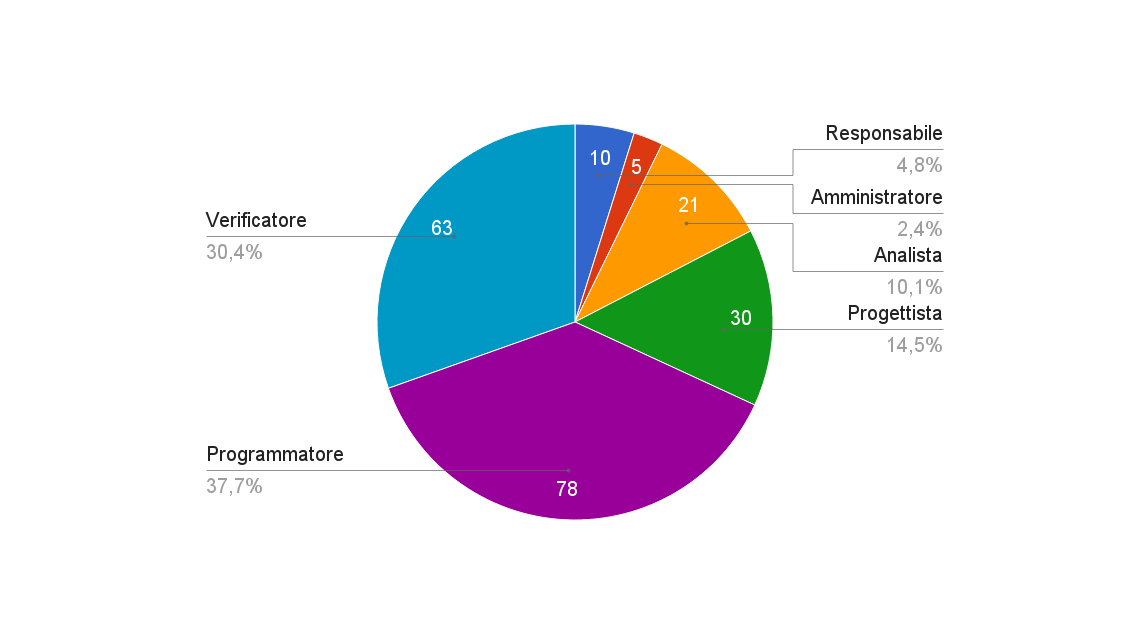
\includegraphics[height=8cm, width=14cm]{img/percOre/PercentualeOreFasePDC.png} 
				\caption{Percentuale di ore per ruolo - Fase PDC}
			\end{figure}
			
				
		
		\subsubsection{Fase RD}	
			\paragraph{Suddivisione del lavoro}
			Nella seguente tabella è descritta la divisione del lavoro nella fase RD:
			\begin{tabella}{!{\VRule}c!{\VRule}c!{\VRule}c!{\VRule}c!{\VRule}c!{\VRule}c!{\VRule}c!{\VRule}c!{\VRule}}
				
				\intestazioneeightcol{Nome}{RE}{AM}{AN}{PG}{PR}{VR}{Ore totali}
				
				Viviana Alessio & - & 3 & - & - & - & 7 & 10 \\
				Enrico Bellio & 6 & - & - & 6 & - & 0 & 12 \\
				Matteo Franco & - & - & - & 3 & 10 & - & 13 \\
				Andrea Grendene & - & - & - & - & - & 11 & 11 \\
				Tommaso Panozzo & - & - & - & 5 & 5 & 2 & 12 \\
				Luca Soldera  & - & - & - & - & 10 & - & 10 \\
				
				\hiderowcolors
				\caption{Ore per componente - Fase RD}
				
			\end{tabella}
			
			\ist{img/istogrammiOre/istRD}{Istogramma ruoli - Fase RD}

			
			\paragraph{Prospetto economico}
			Nella seguente tabella sono riportati i costi relativi alla fase RD da rendicontare al Proponente: 
			\begin{tabella}{!{\VRule}c!{\VRule}c!{\VRule}c!{\VRule}}
				\intestazionethreecol{Ruolo}{Ore}{Costo}
				
				Responsabile & 6 & 180\euro \\
				Amministratore & 3 & 60\euro \\
				Analista & - & - \\
				Progettista & 14 & 308\euro \\
				Programmatore & 25 & 375\euro \\
				Verificatore & 20 & 300\euro \\
				\hline
				\textbf{Totale} & \textbf{68} & \textbf{1223\euro} \\
				\hiderowcolors
				\caption{Ore per ruolo - Fase RD}
			\end{tabella}
			
			\torta{img/percSoldi/percSoldiRD.png}{Percentuale di costo per ruolo sul totale - Fase RD}	
			\torta{img/percOre/PercentualeOreFaseRD.png}{Percentuale di ore per ruolo sul totale - Fase RD}
			
		
		\subsubsection{Fase V}
			\paragraph{Suddivisione del lavoro}
			Nella seguente tabella è descritta la divisione del lavoro nella fase V:
			\begin{tabella}{!{\VRule}c!{\VRule}c!{\VRule}c!{\VRule}c!{\VRule}c!{\VRule}c!{\VRule}c!{\VRule}c!{\VRule}}
				
				\intestazioneeightcol{Nome}{RE}{AM}{AN}{PG}{PR}{VR}{Ore totali}
				
				Viviana Alessio & - & 3 & - & - & - & 12 & 15 \\
				Enrico Bellio & - & 5 & - & - & - & 8 & 13 \\
				Matteo Franco & - & - & - & 3 & - & 10 & 13 \\
				Andrea Grendene & 5 & - & - & - & - & 10 & 15 \\
				Tommaso Panozzo & - & - & - & 5 & 5 & 3 & 13 \\
				Luca Soldera  & - & - & 5 & - & 6 & 3 & 14 \\
				
				\hiderowcolors
				\caption{Ore per componente - Fase V}
				
			\end{tabella}
			
			\ist{img/istogrammiOre/istRD}{Istogramma ruoli - Fase V}		

			
			\paragraph{Prospetto economico}
			Nella seguente tabella sono riportati i costi relativi alla fase V da rendicontare al Proponente: 
			\begin{tabella}{!{\VRule}c!{\VRule}c!{\VRule}c!{\VRule}}
				\intestazionethreecol{Ruolo}{Ore}{Costo}
				
				Responsabile & 5 & 150\euro \\
				Amministratore & 8 & 160\euro \\
				Analista & 5 & 125\euro \\
				Progettista & 8 & 176\euro \\
				Programmatore & 11 & 165\euro \\
				Verificatore & 46 & 690\euro \\
				\hline
				\textbf{Totale} & \textbf{83} & \textbf{1466\euro} \\
				\hiderowcolors
				\caption{Ore per ruolo - Fase V}
			\end{tabella}
			
			\torta{img/percSoldi/percSoldiV.png}{Percentuale di costo per ruolo sul totale - Fase V}	
			\torta{img/percOre/PercentualeOreFaseV.png}{Percentuale di ore per ruolo sul totale - Fase V}
			
	\subsection{Riepilogo}
		\subsubsection{Ore investite}
		
		
		\subsubsection{Ore rendicontate}
	
	


\appendix
\section{Organigramma}
	\subsection{Redazione}
	\begin{tabella}{!{\VRule}c!{\VRule}c!{\VRule}c!{\VRule}}
		\intestazionethreecol{Nominativo}{Data di redazione}{Firma}
		% tanto per salvarmi come fare a includere le immagini delle firme
		Viviana Alessio & 2016/03/19 & \\
	\end{tabella}
	
	\subsection{Approvazione}
	\begin{tabella}{!{\VRule}c!{\VRule}c!{\VRule}c!{\VRule}}
		\intestazionethreecol{Nominativo}{Data di approvazione}{Firma}
		Viviana Alessio & 2016/04/18 &   \\
		Tullio Vardanega & 2016/04/18 &   \\
	\end{tabella}
	
	\subsection{Accettazione dei componenti}
	\begin{tabella}{!{\VRule}c!{\VRule}c!{\VRule}c!{\VRule}}
		\intestazionethreecol{Nominativo}{Data di accettazione}{Firma}
		Viviana Alessio & 2016/04/18 &   \\ 
		Enrico Bellio & 2016/04/18 &   \\
		Matteo Franco & 2016/04/18 &  
\includegraphics[scale=0.1]{img/firme/matteo}\\
		Andrea Grendene & 2016/04/18 &   \\
		Tommaso Panozzo & 2016/04/18 &   \\
		Luca Soldera & 2016/04/18 &   \\
	\end{tabella}	
	
	\subsection{Componenti}
	\begin{tabella}{!{\VRule}c!{\VRule}c!{\VRule}c!{\VRule}}
		\intestazionethreecol{Nominativo}{Matricola}{Indirizzo e-mail}{}
		Viviana Alessio & 1029720 & viviana.alessio@studenti.unipd.it  \\
		Enrico Bellio & 1070872 & enrico.bellio@studenti.unipd.it  \\
		Matteo Franco & 1027207 & matteo.franco.2@studenti.unipd.it  \\
		Andrea Grendene & 1071863 & andrea.grendene@studenti.unipd.it  \\
		Tommaso Panozzo & 1029174 & tommaso.panozzo@studenti.unipd.it  \\
		Luca Soldera & 1028464 & luca.soldera@studenti.unipd.it  \\
	\end{tabella}

\end{document}
